%!TEX root = lab2.tex

\setcounter{chapter}{1}
\chapter{Transport Layer Protocols: \ac{udp} and \ac{tcp}}

What you will learn in this lab:
\begin{itemize}
	\item The differences between data transfers with \ac{udp} and with \ac{tcp}
	\item What effect \acs{ip} Fragmentation has on \ac{tcp} and \ac{udp}
	\item How to analyse measurements of a \ac{tcp} connection
	\item How \ac{tcp} performs retransmissions
	\item How \ac{tcp} congestion control works
	\item How (un)fair bandwidth is divided between multiple \ac{tcp} and \ac{udp} streams
\end{itemize}

\newpage
\section{Lab 2}\label{sec:lab2}

This lab explores the operation of the \acf{tcp} and the \acf{udp}, two of the major transport protocols of the Internet protocol architecture.

\ac{udp} is a simple protocol for exchanging messages from a sending application to a receiving application. \ac{udp} adds a small header to the message, and the resulting data unit is called a \ac{udp} datagram. When a \ac{udp} datagram is transmitted, the datagram is encapsulated in an \acs{ip} header and delivered to its destination. There is one \ac{udp} datagram for each application message.

The operation of \ac{tcp} is more complex. First, \ac{tcp} is a connection-oriented protocol, where a \ac{tcp} client establishes a logical connection to a \ac{tcp} server, before data transmission can take place. Once a connection is established, data transfer can proceed in both directions. The data unit of \ac{tcp}, called a \ac{tcp} segment, consists of a \ac{tcp} header and payload which contains application data. A sending application submits data to \ac{tcp} as a single stream of bytes without indicating message boundaries in the byte stream. The \ac{tcp} sender decides how many bytes are put into a segment.

\ac{tcp} ensures reliable delivery of data, and uses checksums, sequence numbers, acknowledgements, and timers to detect damaged or lost segments. The \ac{tcp} receiver acknowledges the receipt of data by sending an \ac{ack}. Multiple \ac{tcp} segments can be acknowledged in a single \ac{ack}. When a \ac{tcp} sender does not receive an \ac{ack}, the data is assumed lost, and is retransmitted.

\ac{tcp} has two mechanisms that control the amount of data that a \ac{tcp} sender can transmit. First, a \ac{tcp} receiver informs the \ac{tcp} sender how much data it may transmit. This is called flow control. Second, when the network is overloaded and \ac{tcp} segments are lost, the \ac{tcp} sender reduces the rate at which it transmits traffic. This is called congestion control.

The lab covers the main features of \ac{udp} and \ac{tcp}. Part 1 compares the performance of data transmissions in \ac{tcp} and \ac{udp}. Part 2 explores how \ac{tcp} and \ac{udp} deal with \acs{ip} fragmentation. The remaining parts address important aspects of \ac{tcp}. Part 3 explores connection management, Parts 4 and 5 look at flow control and acknowledgements, Part 6 explores retransmissions, and Part 7 is devoted to congestion control. Finally, Part 8 looks into fairness between different \ac{udp} and \ac{tcp} streams.

\newpage
\subsection{Learning how to use iperf}

The \incommand{iperf3} command is a tool used to generate \ac{udp} and \ac{tcp} traffic loads. Together with \incommand{ping6} and \incommand{traceroute6}, \incommand{iperf3} is an essential utility program for debugging problems in \acs{ip} networks. Running the \incommand{iperf3} tool consists of setting up a iperf server (receiver) on one host and then a iperf client (sender) on another host. Once the iperf client is started, it sends the specified amount of data as fast as possible to the iperf server.

\remark Note that both the \incommand{iperf} and the \incommand{iperf3} commands exist. For the remainder of the lab exercises \textbf{do not use \incommand{iperf}, but always use \incommand{iperf3}}, unless specifically stated otherwise!

Some useful \incommand{iperf3} commands:
\begin{framed}
	\begin{itemize}
		\item \incommand{iperf3 -s}\newline Starts an iperf server that  listens for traffic on the default iperf port.
		\item \incommand{iperf3 -c \ipaddr{fc00::1}}\newline Starts an iperf client that sends \acs{tcp} traffic to \ipaddr{fc00::1} on the default port for 10 seconds.
	\end{itemize}
\end{framed}

Refer to the manual page of \incommand{iperf3} for more options.

By default, iperf transmits data over a \ac{tcp} connection. The iperf client opens a \ac{tcp} connection to an iperf server, transmits data and then closes the connection. The iperf server must be running when the iperf client is started. \ac{udp} data transfer is specified with the \incommand{-u} option.

Using the \incommand{-l [bytes]} option tells \incommand{iperf} to send bursts with a set amount of bytes. \ac{udp} sends these bursts as soon as they are presented to the Linux kernel. For \ac{tcp} packets, the Linux kernel can wait a small period of time to group more data together.

The network setup in Figure \ref{fig:lab2-network-topology1} and Table \ref{tab:lab2-mininet1-ip-addresses} is used in part 1 of this lab.

\begin{figure}[ht]
	\centering
	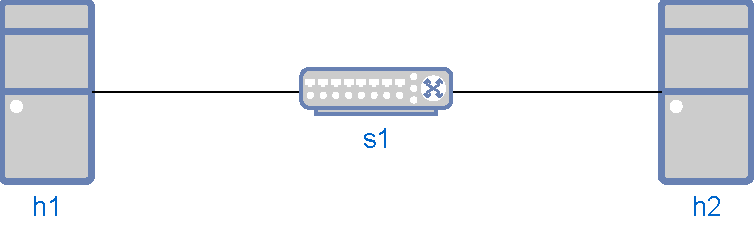
\includegraphics[width=.5\linewidth]{graphics/Lab2-Mininet1}	
	\caption{Network Topology for Part 1.}	
	\label{fig:lab2-network-topology1}
\end{figure}

\begin{table}[ht]
	\centering
	\begin{tabular}{| c | c | c |}	
		\hline
		\textbf{Linux PC} & \textbf{Ethernet Interface eth0} \\ \hline
		h1 & \ipaddr{fc00:0:0:1::1/64} \\ 
		h2 & \ipaddr{fc00:0:0:1::2/64} \\ \hline
	\end{tabular}
	\caption{\acs{ip} Addresses of the hosts.}
	\label{tab:lab2-mininet1-ip-addresses}
\end{table}

\begin{exercise}{Network setup}
\label{ex:udp-iperf}
\begin{enumerate}
	\item Write a mininet python script to create the topology as shown in Figure \ref{fig:lab2-network-topology1}, and save it as \linktrace[1]{py}. Configure the \acs{ip} addresses of the interfaces as given in Table \ref{tab:lab2-mininet1-ip-addresses}.
	\item Run the mininet script.
	\item Verify that the setup is correct by issuing a \incommand{pingall} command in mininet.
\end{enumerate}
\end{exercise}


\begin{exercise}{Transmitting data with \ac{udp}}
This exercise consists of setting up a \ac{udp} data transfer between two hosts, h1 and h2, and observe the \ac{udp} traffic.

\begin{enumerate}
	\item Open xterm terminals on both h1 and h2.
	\item On h1, start Wireshark and start capturing packets on the \incommand{h1-eth0} interface. 
	\item On h2, start an iperf server.
	\item On h1, start a iperf client that transmits \ac{udp} traffic to h2. Limit the length of the buffer to send to 500 bytes, and limit the total amount of bytes to send to 10000. 
	\item Stop the Wireshark capture on h1 and save the captured traffic to \file[1]{pcapng}.
	\item For the following questions, filter out \ac{udp} traffic with a display filter and ignore the first small 4 byte packet or packets; this is a sort of "handshake" that iperf3 is performing and has nothing to do with the actual data transfer.
\end{enumerate}

\textbf{Use the data captured with Wireshark in \linktrace[1]{pcapng} to answer the questions. Support your answers with the saved Wireshark data.}

\question{How many packets are exchanged in the data transfer? How many \ac{ip} packets are transmitted for each \ac{udp} datagram? What is the size of the \ac{udp} payload of these packets?}{1}
\question{Compare the total number of bytes transmitted, in both directions, including Ethernet, \ac{ip}, and \ac{udp} headers, to the amount of application data transmitted.}{1}
\question{Explain the fields in the \ac{udp} headers.}{1}
\question{Observe the port numbers in the \ac{udp} header. How did the iperf client select the source port number?}{1}

\end{exercise}

\newpage
\subsection{\acs{ip} Fragmentation of \ac{udp} traffic}

In this part of the lab, you observe the effect of \acs{ip} fragmentation on \ac{udp} traffic. Fragmentation occurs when the transport layer sends a packet of data to the \acs{ip} layer that exceeds the \acf{mtu} of the underlying data link network. For example, in Ethernet networks, the \ac{mtu} typically is 1500 bytes. If an \acs{ip} datagram exceeds the \ac{mtu} size, an error message is reported and the original packet has to be split into smaller packets.

When a \acs{udp} datagram is fragmented, its payload is split into multiple \acs{ip} packets, each satisfying the limit imposed by the \ac{mtu}. Each fragment is an independent \acs{ip} packet, and is routed in the network independently from the other fragments. Fragmentation only happens at the sending host. Intermediate hops are not allowed to fragment \acs{ipv6} packets (in \acs{ipv4} this is different - this will be shown in another lab). Fragments are reassembled only at the destination host.

Even though \acs{ip} fragmentation provides flexibility that can hide differences of data link technologies to higher layers, it incurs considerable overhead, and, therefore, should be avoided.

\begin{figure}[ht]
	\centering
	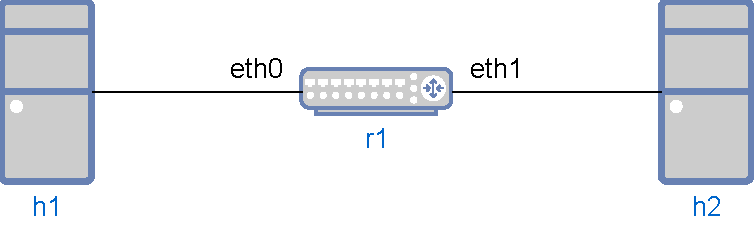
\includegraphics[width=.5\linewidth]{graphics/Lab2-Mininet2}	
	\caption{Network Topology for Part 2.}
	\label{fig:lab2-network-topology2}
\end{figure}

\begin{table}[ht]
	\centering
	\begin{tabular}{| c | c | c |}	
		\hline
		\textbf{Linux PC} & \textbf{Ethernet Interface eth0} & \textbf{Ethernet Interface eth1} \\ \hline
		h1 & \ipaddr{fc00:0:0:1::1/64} & N/A \\
		h2 & \ipaddr{fc00:0:0:2::2/64} & N/A \\
		r1 & \ipaddr{fc00:0:0:1::10/64} & \ipaddr{fc00:0:0:2::10/64} \\ \hline
	\end{tabular}
	\caption{\acs{ip} Addresses of the hosts and router.}
	\label{tab:lab2-mininet2-ip-addresses}
\end{table}

You explore the issues with \acs{ip} fragmentation of \ac{udp} transmissions in the network configuration shown in Figure \ref{fig:lab2-network-topology2}, with h1 as sending host, h2 as receiving host, and r1 as intermediate \acs{ip} router.

\begin{exercise}{\ac{udp} and Fragmentation}
In this exercise you observe \acs{ip} fragmentation of \ac{udp} traffic. In the following exercise, use \incommand{iperf3} to generate \ac{udp} traffic between h1 and h2, across \acs{ip} router r1.

\begin{enumerate}
	\item Write a python script that sets up the mininet topology shown in \ref{fig:lab2-network-topology2}. Make sure you configure the IP addresses as shown in table \ref{tab:lab2-mininet2-ip-addresses}. Save the script to \linktrace[1]{py}.
	\item Start mininet and verify that the network is configured correctly by issuing a \incommand{pingall}.
	\item Start Wireshark on the \incommand{h1-eth0} interface of h1 and start to capture traffic. Do not set any filters.
	\item Use \incommand{iperf3} to generate \ac{udp} traffic between h1 and h2. The connection parameters are selected so that \acs{ip} Fragmentation does not occur initially:
	\begin{itemize}
		\item Start an \incommand{iperf3} server on h2.
		\item On h1, start an iperf3 client that transmits \ac{udp} traffic to h2. Limit the length of the buffer to send to 1000 bytes, and limit the total amount of bytes to send to 10000.
	\end{itemize}
	\item Next, try sending larger datagrams by issuing the previous \incommand{iperf} command again, but this time, instead of \incommand{1000}, choose \incommand{2000} as buffer length.
	\item Stop the traffic capture on h1 and save the Wireshark output to \file[1]{pcapng}.
\end{enumerate}

\remark Wireshark reassembles fragmented \ac{ip} packets by default. In order to actually see what is going on without Wireshark reassembling, verify the following settings in Wireshark (you should keep the same settings for all future labs as well):
\begin{itemize}
	\item Preferences -> Advanced -> ipv6.defragment: \textbf{FALSE}.
	\item Preferences -> Advanced -> ip.defragment: \textbf{FALSE}.
	\item Preferences -> Protocols -> IPv6 -> Reassemble IPv6 datagrams: \textbf{OFF}.
	\item Preferences -> Protocols -> IPv4 -> Reassemble IPv4 datagrams: \textbf{OFF}.
\end{itemize}

\textbf{Use the data captured with Wireshark in \linktrace[1]{pcapng} to answer the questions. Support your answers with the saved Wireshark data.}

\question{From the saved Wireshark data, select one \acs{udp} datagram that is fragmented. For each fragment of this datagram, determine the values of the fields in the \acs{ip} fragmentation header.}{1}
\question{What is the maximum size of an \ac{udp} datagram that does not require fragmentation? What is the amount of actual data that is transmitted in such a datagram?}{1}
\question{For the iperf session that resulted in fragmented datagrams: How large is the first datagram? How large is the second? How much application data is in both fragments?}{1}
\question{Why don't intermediate routers reassemble fragmented \acs{ip} packets?}{1}
\end{exercise}

\begin{exercise}{The effect of fragmentation on performance.}
For this exercise, we start from the same topology as we used in the previous exercise. However, in order to avoid dealing with very large trace files, we will modify the topology a bit so the links between the router and the hosts is capped to 1Mbps. You can do this by supplying an extra argument \incommand{bw=X} to the \incommand{addlink} methods in your python script, where X is the bandwidth of the link expressed in Mbps:
\begin{cmdblock}[gobble=3]
	% addLink(h1, r1, bw=1)
\end{cmdblock}
\begin{enumerate}
	\item Modify your python script so the links are set to 1Mbps and save it as \linktrace[1]{py}.
	\item Once again, start mininet and verify the connectivity with the \incommand{pingall} command.
	\item Start an iperf server on h2.
	\item Start capturing packets with wireshark on h1.
	\item On h1, start an iperf session to h2. The parameters for the iperf session this time are:
	\begin{itemize}
		\item Make iperf run for 10 seconds and then stop.
		\item Set the target bandwidth to 1Mbps. This ensures we will completely fill the link to its maximum capacity.
		\item Use \ac{udp}
		\item Limit the buffer length to 1452.
	\end{itemize}
	\item Save the output of the iperf server to \file[1]{txt} and the wireshark trace to \file[1]{pcapng}.
	\item Start a new wireshark session on h1.
	\item Run the same iperf command again on h1, but this time use a buffer length of 1453.
	\item Save the output of the iperf server to \file[2]{txt} and the wireshark trace to \file[2]{pcapng}.
	\item Again start a new wireshark session on h1, and run the same iperf command, but now use 2778 as buffer length.
	\item Save the output of the iperf server to \file[3]{txt} and the wireshark trace to \file[3]{pcapng}.
	\item Finally, repeat the same steps again to run an iperf session with a buffer length of 2115. Save the outputs again to \file[4]{txt} and the wireshark trace to \file[4]{pcapng}.
\end{enumerate}

\textbf{Use the data captured in \linktrace[1]{txt}, \linktrace[2]{txt}, \linktrace[3]{txt}, \linktrace[4]{txt}, \linktrace[1]{pcapng}, \linktrace[2]{pcapng}, \linktrace[3]{pcapng} and \linktrace[4]{pcapng} to answer the questions. Support your answers with the saved Wireshark data and iperf output.}

\question{Look at the summary line of iperf3 that displays the throughput throughout the entire 10 second session. Look at the \textbf{receiver} report! Compare the throughput of the four iperf sessions. How much difference is there between the biggest and lowest reported throughput?}{1}
\question{Explain why not every session results in the same throughput. Use your wireshark traces to support your answer.}{1}
\question{One of the sessions will have the lowest reported throughput. Why that specific session?}{1}
\end{exercise}

\newpage
\subsection{\ac{tcp} and iperf}
Up until now, we have been using \incommand{iperf3} over \ac{udp}. The next parts of the lab will focus on the behaviour of \ac{tcp}. As you will see, \ac{tcp} is a \emph{connection-oriented} protocol, in contrast to \ac{udp}, which is \emph{connectionless}. Moreover, \ac{tcp} provides reliable, ordered and error-checked delivery of data. In the next exercises, all these concepts will be touched upon. We will start by running a simple iperf session, as we did with \ac{udp}.

\begin{exercise}{Transmitting data with \ac{tcp}}
Use the same topology as shown in figure \ref{fig:lab2-network-topology2} and table \ref{tab:lab2-mininet2-ip-addresses}.\\
\remark \textbf{In order to interpret the results in this exercise correctly, it is necessary to make another slight modification to the python script!} Right after the \incommand{net.start()} line, insert the following line: \incommand{net["h1"].cmd("ethtool -K h1-eth0 tso off")}. Save your modified script to \file{py}.

The reason for this change is because by default \emph{\acs{tcp} segmentation offload} or \emph{tso} is enabled on Linux systems. This is a technology where (parts of) the \acs{tcp}/\acs{ip} processing is offloaded to the network controller. This technique reduces the processing overhead of the network stack on the CPU. However, when it is enabled, your operating system typically ``sees'' (much) larger packets than are actually sent on the network hardware (less, but larger packets = less processing overhead). The network card then does the \emph{actual} processing. This can be misleading when you look at your wireshark traces because you don't see what is actually happening on the network. You see what the CPU of your machine \emph{thinks} is happening\ldots.

Therefore, it is recommended to turn this technique off for exercises where this matters. For the remainder of the course, when its is mentioned to turn off tso or TCP segmentation offload, you are expected to insert a similar line in your python scripts. When nothing is mentioned, turning off tso is not required (but it is OK if you always turn it off by default in your scripts).

\remark This is one of the few exercises where you \textbf{must use iperf instead of iperf3}. Read up on the man page of iperf as the syntax is slightly different from iperf3!

\begin{enumerate}
	\item On h1, start Wireshark and start capturing packets on the network interface of h1. 
	\item On h2, start an iperf server. 
	\item Start a iperf client on h1 that transmits \ac{tcp} packets to h2. Limit the total amount of bytes to send to 10000. 
	\item Stop the wireshark capture on h1, and save the captured traffic to \file[1]{pcapng}.
\end{enumerate}

\textbf{Use the data captured with Wireshark in \linktrace[1]{pcapng} to answer the questions.}

\question{How many packets contain application data? How many bytes of application data do those packets contain?}{1}
\question{Compare the total number of bytes transmitted, in both directions, including Ethernet, IP, and \ac{tcp} headers, to the amount of application data transmitted.}{1}
\question{Inspect the \ac{tcp} headers. Which packets contain flags in the \ac{tcp} header? Which types of flags do you observe and what is their purpose?}{1}
\question{Compare the total amount of bytes transmitted in this \ac{tcp} data transfer, and the \ac{udp} data transfer in exercise \ref{ex:udp-iperf}.}{1}

\end{exercise}

\newpage
\subsection{\ac{tcp} and Fragmentation}

\begin{exercise}{\ac{tcp} and Fragmentation}
\ac{tcp} avoids fragmentation with the following two mechanisms:

\begin{itemize}
	\item When a \ac{tcp} connection is established, it negotiates the \acf{mss}. Both the \ac{tcp} client and the \ac{tcp} server send the \ac{mss} in an option that is attached to the \ac{tcp} header of the first transmitted \ac{tcp} segment. Each side sets the \ac{mss} so that no fragmentation occurs at the outgoing network interface, when it transmits segments. The smaller value is adopted as the \ac{mss} value for the connection.
	\item The exchange of the \ac{mss} only addresses \ac{mtu} constraints at the hosts, but not at the intermediate routers. To determine the smallest \ac{mtu} on the path from the sender to the receiver, \ac{tcp} employs a method that is known as Path \ac{mtu} Discovery, and that works as follows: when a router can't forward a packet because it is larger than the \ac{mtu} of the link, it discards the packet and generates an \ac{icmp} error message of type ``Packet Too Big'' (in \acs{ipv6}) or ``Fragmentation needed; DF bit set'' (in \acs{ipv4}). Upon receiving such an \ac{icmp} error message, the \ac{tcp} sender reduces the segment size. This continues until a segment size is determined which does not trigger an \ac{icmp} error message.
\end{itemize}

\begin{table}[ht]
	\centering
	\begin{tabular}{ | c | c | c | }	
		\hline
		\textbf{Linux PC} & \textbf{\ac{mtu} size of eth0} & \textbf{\ac{mtu} size of eth1} \\ \hline
		h1 & 1500 & N/A \\ 
		h2 & 1280 & N/A \\
		r1 & 1500 & 1500 \\ \hline
	\end{tabular}
	\caption{\ac{mtu} Sizes}
	\label{tab:lab5-mtus}
\end{table}

For this exercise, continue to use the same python script as in the previous exercise. Once you have started up the script, perform the steps mentioned below.

\remark You should switch back to using \incommand{iperf3} for this exercise!
\begin{enumerate}
	\item Modify the \ac{mtu} of the interfaces with the values as shown in Table \ref{tab:lab5-mtus}. In Linux, you can view the \ac{mtu} values of all interfaces in the output of the \incommand{ifconfig} command. For example, on h2, you type:
	\begin{cmdblock}[gobble=2]
		h2% ifconfig
	\end{cmdblock}
	The same command is used to modify the \ac{mtu} value. For example, to set the \ac{mtu} value of interface h2-eth0 on h2 to 1280 bytes, use the \incommand{ifconfig} command as follows:
	\begin{cmdblock}[gobble=2]
		h2% ifconfig h2-eth0 mtu 1280
	\end{cmdblock}
	\item Start Wireshark on h1 and start to capture traffic with no filters set.
	\item \label{step:lab5-tcpfrag-client} Start an iperf server on h2, and an iperf client on h1 that sends \ac{tcp} packets to h2. Limit the duration of the iperf session to 1 second.
	\item Save the Wireshark output to \file[1]{pcapng}. 
	\item Now change the \ac{mtu} size on interface eth1 of r1 to 1280 bytes. Change the \ac{mtu} size of interface eth0 on h2 to 1500 bytes.
	\item Start Wireshark on h1 again.
	\item Repeat the iperf transmission in step \ref{step:lab5-tcpfrag-client}.
	\item Save the Wireshark output to \file[2]{pcapng}.
\end{enumerate}

\remark When answering the following questions, take into account that \incommand{iperf3} actually sets up \textbf{two} \acs{tcp} connections: the first one is always a control connection over which client and server exchange statistics etc. This \acs{tcp} connection is also present when you perform a \acs{udp} iperf. In the case of a \acs{tcp} \incommand{iperf3}, the \emph{second} \acs{tcp} connection is the one that is doing the actual data transmission!

\textbf{Use the data captured with Wireshark in \linktrace[1]{pcapng} to answer the following questions.}

\question{Do you observe fragmentation before changing the \ac{mtu} on r1? If so, where does it occur? If not, why not? Explain your observation.}{2}

\textbf{Use the data captured with Wireshark in \linktrace[2]{pcapng} to answer the following questions.}

\question{Do you observe fragmentation after changing the \ac{mtu} on r1? If so, where does it occur? Explain your observation.}{1}
\question{Describe how Path \ac{mtu} Discovery is performed.}{1}

\end{exercise}


\newpage
\subsection{\ac{tcp} connection management}

\ac{tcp} is a connection-oriented protocol. The establishment of a \ac{tcp} connection is initiated when a \ac{tcp} client sends a request for a connection to a \ac{tcp} server. The \ac{tcp} server must be running when the connection request is issued.

\ac{tcp} requires three packets to open a connection. This procedure is called a three-way handshake. During the handshake the \ac{tcp} client and \ac{tcp} server negotiate essential parameters of the \ac{tcp} connection, including the initial sequence numbers, the maximum segment size, and the size of the windows for the sliding window flow control. \ac{tcp} requires three or four packets to close a connection. Each end of the connection is closed separately, and each part of the closing is called a half-close.

\ac{tcp} does not have separate control packets for opening and closing connections. Instead, \ac{tcp} uses bit flags in the \ac{tcp} header to indicate that a \ac{tcp} header carries control information. The flags involved in the opening and the closing of a connection are: SYN, ACK, and FIN.

Here, you use ssh to set up a \ac{tcp} connection and observe the control packets that establish and terminate a \ac{tcp} connection. The experiments involve h1 and h2 in the same network as shown in Figure \ref{fig:lab2-network-topology2}. You can continue to use the python script from the previous exercise.

\begin{exercise}{Opening and Closing a \ac{tcp} Connection}
Set up a \ac{tcp} connection and observe the packets that open and close the connection. Determine how the parameters of a \ac{tcp} connection are negotiated between the \ac{tcp} client and the \ac{tcp} server.

\begin{enumerate}
	\item This part of the lab only uses h1 and h2 in the network configuration in Figure \ref{fig:lab2-network-topology2}.
	Verify that the \ac{mtu} values of all interfaces of h1, and h2, and r1 are set to 1500 bytes, which is the default \ac{mtu} for Ethernet networks.
	\item Start Wireshark on h1 to capture traffic of the ssh connection. Do not set any filters.
	\item Start up the ssh daemon on h2 as follows:
	\begin{cmdblock}[gobble=2]
		h2% /sbin/sshd
	\end{cmdblock}
	\item Establishing a \ac{tcp} connection: Establish a ssh session from h1 to h2. Use the username ``computernetwerken'' and the password for the VM to log in on h2.
	\item Closing a \ac{tcp} connection (initiated by client): On h1, type \incommand{exit} in the ssh session to terminate the connection.
	\item Save the Wireshark output as \file{pcapng}.
\end{enumerate}

\textbf{Use the data captured with Wireshark in \linktrace[1]{pcapng} to answer the following questions.}

\question{Identify the packets of the three-way handshake (refer to the frame numbers). Which flags are set in the \ac{tcp} headers? Explain how these flags are interpreted by the receiving \ac{tcp} server or \ac{tcp} client.}{1}
\question{During the connection setup, the \ac{tcp} client and \ac{tcp} server tell each other the first sequence number they will use for data transmission. What is the initial sequence number chosen by h1 and h2? How is this initial sequence number chosen?}{1}
\question{Identify the first packet that contains data. What is the sequence number used in the first byte of data sent from the \ac{tcp} client to the \ac{tcp} server?}{1} 
\question{Identify the packets that are involved in closing the \ac{tcp} connection. Which flags are set in these packets? Explain how these flags are interpreted by the receiving \ac{tcp} server or \ac{tcp} client.}{1}
\end{exercise}

\newpage
\subsection{Retransmissions in \ac{tcp}}
Next you observe retransmissions in \ac{tcp}. \ac{tcp} uses ACKs and timers to trigger retransmissions of lost segments. A \ac{tcp} sender retransmits a segment when it assumes that the segment has been lost. This occurs in two situations:

\begin{enumerate}
	\item No ACK has been received for a segment. Each \ac{tcp} sender maintains a retransmission timer for the connection. When the timer expires, the \ac{tcp} sender retransmits the earliest segment that has not been acknowledged. The timer is started when a segment with payload is transmitted and the timer is not running, when an ACK arrives that acknowledges new data, and when a segment is retransmitted. The timer is stopped when all outstanding data has been acknowledged.
	
	The retransmission timer is set to a \acf{rto} value, which adapts to the current network delays between the sender and the receiver. A \ac{tcp} connection performs round-trip measurements by calculating the delay between the transmission of a segment and the receipt of the acknowledgement for that segment. The \ac{rto} value is calculated based on these round-trip measurements. Following a heuristic which is called Karn's algorithm, measurements are not taken for retransmitted segments. Instead, when a retransmission occurs, the current \ac{rto} value is simply doubled.
	
	\item Multiple ACKs have been received for the same segment. A duplicate acknowledgement for a segment can be caused by an out-of-order delivery of a segment, or by a lost packet. A \ac{tcp} sender takes multiple, in most cases three, duplicates as an indication that a packet has been lost. In this case, the \ac{tcp} sender does not wait until the timer expires, but immediately retransmits the segment that is presumed lost. This mechanism is known as fast retransmit. The \ac{tcp} receiver expedites a fast retransmit by sending an ACK for each packet that is received out-of-order.
	
	A disadvantage of cumulative acknowledgements in \ac{tcp} is that a \ac{tcp} receiver cannot request the retransmission of specific segments. For example, if the receiver has obtained segments 1, 2, 3, 5, 6, 7 cumulative acknowledgements only permit to send ACK for segments 1, 2, 3 but not for the other correctly received segments. This may result in an unnecessary retransmission of segments 5, 6, and 7. The problem can be remedied with an optional feature of \ac{tcp}, which is known as selective acknowledgement (SACKs). Here, in addition to acknowledging the highest sequence number of contiguous data that has been received correctly, a receiver can acknowledge additional blocks of sequence numbers. The range of these blocks is included in \ac{tcp} headers as an option. Whether SACKs are used or not, is negotiated in \ac{tcp} header options when the \ac{tcp} connection is created.
\end{enumerate}

The exercises in this part explore aspects of \ac{tcp} retransmissions that do not require access to internal timers. Unfortunately, the roundtrip time measurements and the \ac{rto} values are difficult to observe, and are, therefore, not included in this lab.

The network configuration for this part is still the same network as shown in Figure \ref{fig:lab2-network-topology2}.


\begin{exercise}{\ac{tcp} Retransmissions}
The purpose of this exercise is to observe when \ac{tcp} retransmissions occur. As before, you transmit data from h1 to h2. Here, data is sent over a link that is set to 1Mbps and will create a 1\% packet loss. When a packet gets lost, you will see that it gets retransmitted.

\begin{enumerate}
	\item Modify the python script you used in the previous exercise by adding the \incommand{loss=1} to every link, similar to setting the bandwidth cap earlier. Also for this exercise, double-check that the bandwidth is still capped to 1 Mbps. Save your script to \file{py}.
	\item Start Wireshark on h2 and capture traffic on interface h2-eth0. Set a display filter to \ac{tcp} traffic. 
	\item Make sure an iperf server is  running on h2.
	\item On h1, start an iperf client that sends 10 seconds worth of data to h2.
	\item When the data transfer finishes, stop the Wireshark capture and save it to \file{pcapng}
\end{enumerate}

\textbf{Refer to examples in the saved Wireshark data (\linktrace[1]{pcapng}). Include images of graphs where possible.}

When you scroll through the wireshark trace, you will find (probably several) places where retransmits are occurring. You can easily identify these places because wireshark will mark these lines in black and red. Refer to one such an occurrence in your wireshark trace to answer the next questions.
\question{Which packet(s) were lost?}{1}
\question{Which packet(s) were retransmitted?}{1}
\question{How does the sender know the receiver missed one (or more) packets?}{1}
\question{Are only lost packets retransmitted, or are there also other packets that are retransmitted? Why or why not?}{3}
\end{exercise}

\newpage
\subsection{\ac{tcp} Congestion Control}

\ac{tcp} congestion control consists of a set of algorithms that adapt the sending rate of a \ac{tcp} sender to the current conditions in the network. When the network is not congested, the \ac{tcp} sender is allowed to increase its sending rate, and when the network is congested, the \ac{tcp} sender reduces its rate. The \ac{tcp} sender maintains a congestion window which limits the number of segments that can be sent without waiting for an acknowledgement. The actual number of segments that can be sent is the minimum of the congestion window and the window size sent by the receiver.

For congestion control, each \ac{tcp} sender keeps two variables, the congestion window (cwnd) and the slow-start threshold (ssthresh). \ac{tcp} congestion control operates in two phases, called slow start and congestion avoidance. The sender is in the slow start phase when cwnd $\le$ ssthresh. Here, cwnd is increased by one for each arrived ACK. This results in a doubling of cwnd for each roundtrip time. When cwnd $>$ ssthresh, the \ac{tcp} sender is in the congestion avoidance phase. Here, the cwnd is incremented by one only after cwnd ACKs. This is done by incrementing cwnd by a fraction of a segment when an ACK arrives.

The \ac{tcp} sender assumes that the network is congested when a segment is lost, that is, when the retransmission timer has a timeout or when three duplicate ACKs arrive. When a timeout occurs, the \ac{tcp} sender sets ssthresh to half the current value of cwnd and then sets cwnd to one. This puts the \ac{tcp} sender in slow start mode. When a third duplicate ACK arrives, the \ac{tcp} sender performs what is called a fast recovery. Here, ssthresh is set to half the current value of cwnd, and cwnd is set to the new value of ssthresh.

The goal of this part of the lab is to observe the development of the congestion window and to see the slow start and congestion avoidance phases of a \ac{tcp} session.

\begin{exercise}{Observing \ac{tcp} congestion control}
The network configuration used is still that in Figure \ref{fig:lab2-network-topology2}. To observe the slow start features, we will once again apply slight modifications to the python script of the previous exercise to make things easier to follow. We will keep the 1 Mbps bandwidth limit, but we remove the 1\% packet loss that was introduced in the previous exercise. We will now also add a large delay on the links, so that the slow start phase will be lasting longer and is easier to observe. We are going to add 240 ms of delay to the link between r1 and h2, which is more or less equivalent to what would be expected if traffic is routed over a geostationary satellite. You could think of h1 and h2 as ground stations, and r1 as the satellite in this scenario. In order to add delay to a link, similar to capping the bandwidth, we need to add another parameter to that link: \incommand{delay="240ms")}.

When h1 sends a data segment to h2, the ACK for that segment will take about 0.5 seconds to arrive to h1 (240ms delay for the data segment, and the same for the ACK). This spaces out the packets nicely so slow start is easier to follow.


\begin{enumerate}
	\item Modify the python script for the topology so the link between r1 and h2 has a delay of 240 ms, and neither of the links have the 1\% packet loss. Save it to \file{py}.
	\item Start a wireshark capture on h1.
	\item Start an iperf server on h2.
	\item Start an iperf client on h1 that transmits 10 seconds worth of data to h2.
	\item Save your wireshark trace to \file{pcapng}.
\end{enumerate}

\textbf{Refer to examples in the saved Wireshark data (\linktrace[1]{pcapng}). Include images of graphs where possible.}

\begin{figure}[ht]
	\centering
	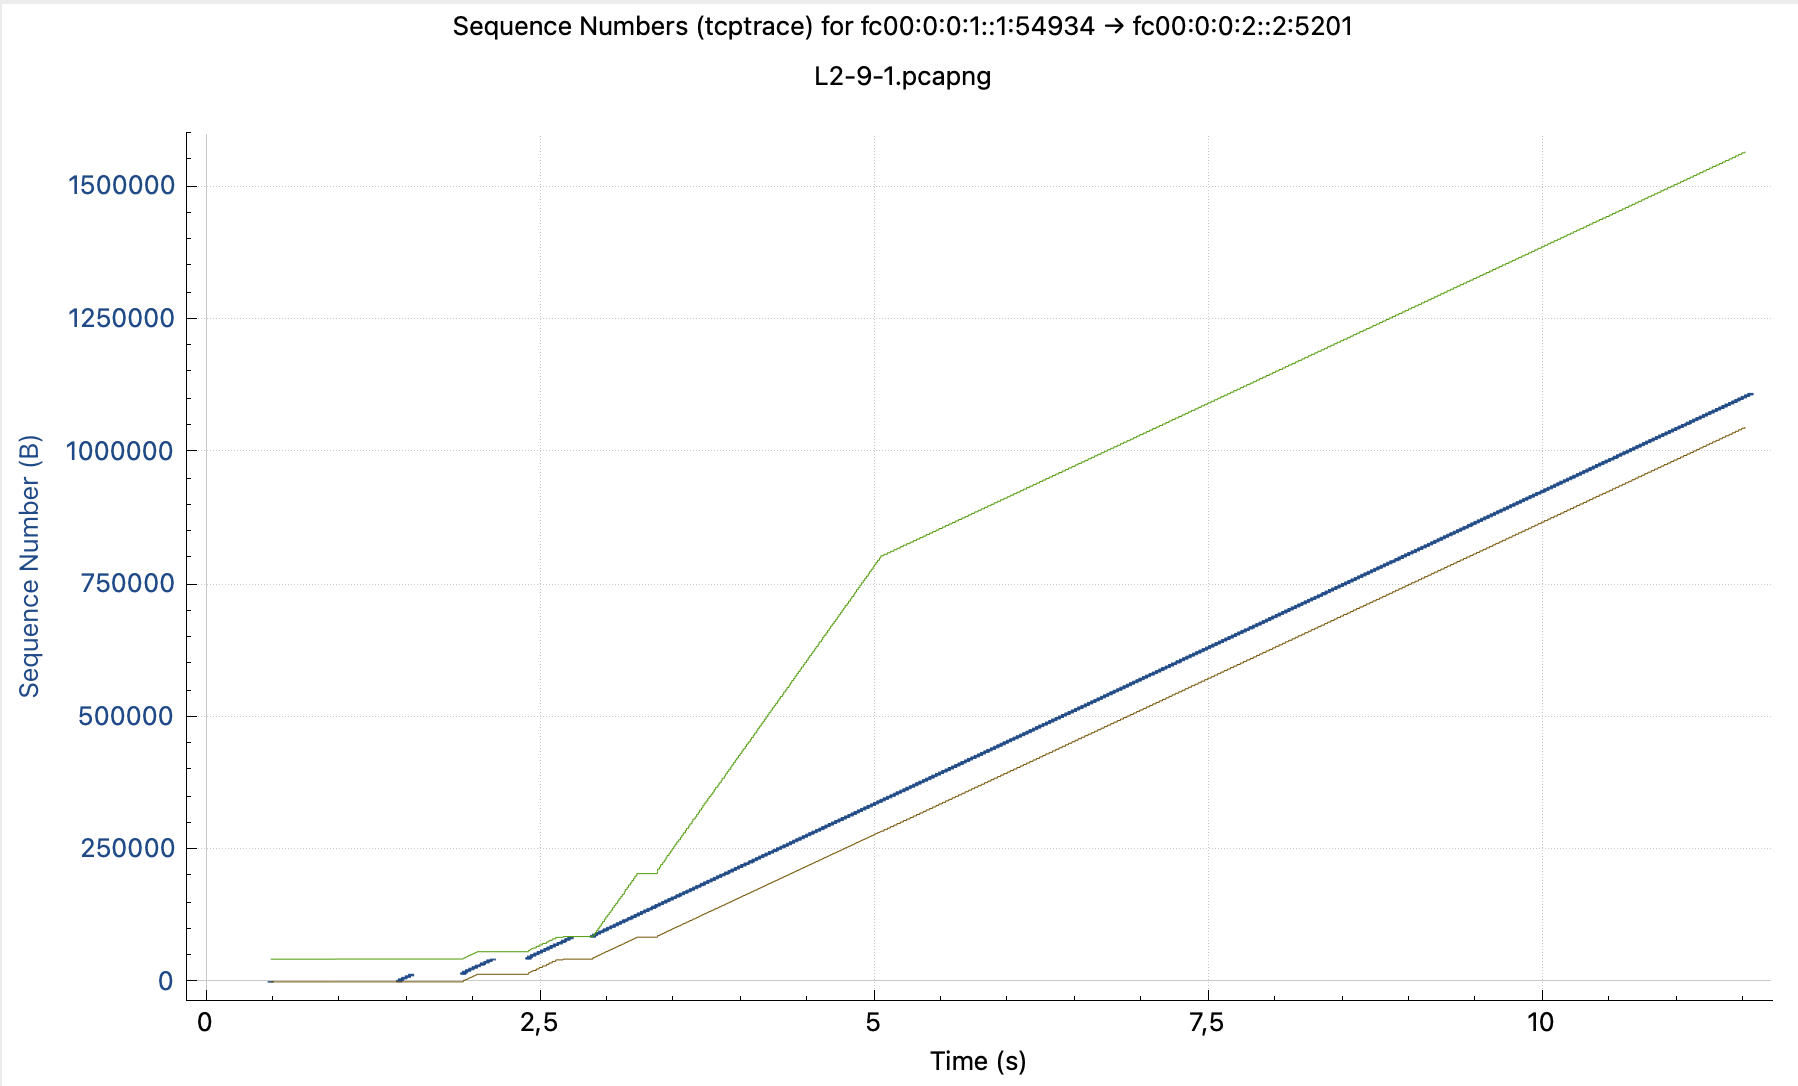
\includegraphics[width=\linewidth]{graphics/Lab2-tcptrace}	
	\caption{tcptrace graph.}	
	\label{fig:lab2-tcptrace}
\end{figure}

\question{In your wireshark trace, select a packet that belongs to the \acs{tcp} iperf session. Select a packet that is sent from h1 towards h2. Next, select \emph{Statistics} -> \emph{TCP Stream Graphs} -> \emph{Time Sequence (tcptrace)}. You should see a graph like in Figure \ref{fig:lab2-tcptrace}. If you don't see a similar graph, check if clicking the ``Switch Direction'' button helps. You can zoom in on the start of the graph to have a closer look at the slow start phase of the TCP session. Export the graph as \incommand{tcptrace.png}. and include it in your report. You can also include extra images of zoomed-in parts of the graph to highlight any details. What is the meaning of the curves on the graph? What do they represent? Using the graph, can you explain how slow start works?}{2}
\question{Using the graph, indicate where the behaviour of the slow start phase changes. How can you tell? What is happening differently after the change?}{2}
\end{exercise}

\newpage
\subsection{Fairness}
\begin{exercise}{Create and perform your own experiments}
For this exercise you are going to create your own experiments that showcase the workings of fairness with \ac{tcp} and \ac{udp}.

\remark When you create this experiment, it is very important that, on \textbf{any link} in your network where you apply \textbf{bandwidth limitations}, you also need to add another, extra parameter to the link: \incommand{enable\_red=True}.

Without that extra parameter, you will encounter a phenomenon known as ``Bufferbloat'', which is a well-known cause of high latency and jitter in packet-switched networks caused by excess buffering of packets. \ac{tcp} uses the occurrence of packet drops to determine the available bandwidth between two hosts. The algorithms speed up the data transfer until packets start to drop, then slow down the transmission rate. Ideally, they keep adjusting the transmission rate until it reaches an equilibrium speed of the link. With a large buffer that has been filled, the packets will arrive at their destination, but with a higher latency. The packets were not dropped, so \ac{tcp} does not slow down once the uplink has been saturated, further filling the buffer. Newly arriving packets are dropped only when the buffer is fully saturated. To \ac{tcp}, a congested link can appear to be operating normally as the buffer fills. The \ac{tcp} algorithm is unaware the link is congested and does not start to take corrective action until the buffer finally overflows and packets are dropped.

A nice article, written by Jim Gettys and Kathleen Nichols, that digs deeper into this problem has been published in the ``Communications of the ACM'' magazine in January 2012, and can be found on \url{https://cacm.acm.org/magazines/2012/1/144810-bufferbloat/fulltext}

How the extra \incommand{enable\_red=True} parameter solves this problem, is out of scope for this exercise.


Your experiment must consist of the following aspects:
\begin{enumerate}
	\item A network topology to run the experiments on.
	\item A description of the steps to perform in order to set up the experiment.
	\item The experiment steps itself.
	\item A conclusion about what you noticed and a callback to the theory about fairness.
\end{enumerate}
As more than one experiment might be needed, steps 2 and 3 can be repeated as much as required.


Make sure you showcase the following situations within your experiments:
\begin{enumerate}
	\item What happens when multiple \ac{tcp} connections are present?
	\item What happens when multiple connections and at least one \ac{udp} stream are present?
	\item How does fairness work with two \ac{tcp} connections, where every connection has a different \ac{rtt}? Can you illustrate this?
\end{enumerate}
When you answer this question, make sure that you write it down so that others can easily reproduce your experiments. People who want to perform your experiments should not make assumptions or guess what they have to do.

Tips:
\begin{enumerate}
	\item To avoid having huge traces in Wireshark, make sure you limit the bandwidth of the links (limiting the bandwidth of one link on the entire path is sufficient).
	\item Some questions may require a different topology. You can make multiple topologies for all experiments.
	\item Always test your network topology before starting to perform the actual experiments. Make sure the topology behaves as you would expect.
	\item Don't forget about the \incommand{tso off} feature!
	\item Make sure you include all relevant python scripts, output, wireshark traces, \ldots in your report.
\end{enumerate}

\question{Describe your complete experiment and conclusions.}{10}
\end{exercise}